\documentclass[a4paper,12pt]{article}

% -------------------------------------------------
% Configuração de página
% -------------------------------------------------
\usepackage[a4paper,
top=3cm,
bottom=2.5cm,
left=3cm,
right=2.5cm]{geometry}

% -------------------------------------------------
% Codificação e idioma
% -------------------------------------------------
\usepackage[T1]{fontenc}
\usepackage[utf8]{inputenc}
\usepackage[english,brazil]{babel}

\usepackage{mathptmx}

% -------------------------------------------------
% Pacotes matemáticos e fontes
% -------------------------------------------------
\usepackage{amsmath}
\usepackage{amsfonts}
\usepackage{amstext}
\usepackage{mathptmx}
\usepackage[normalem]{ulem}

% -------------------------------------------------
% Formatação geral
% -------------------------------------------------
\usepackage{indentfirst}
\usepackage{microtype}
\usepackage{setspace}
\onehalfspacing
\setlength{\parindent}{1.25cm}
\setlength{\parskip}{0pt}

% -------------------------------------------------
% Gráficos, tabelas e quadros
% -------------------------------------------------
\usepackage{graphicx}
\usepackage{graphics}
\usepackage{float}
\usepackage{booktabs}
\usepackage{array}
\usepackage{tabularx}
\usepackage{longtable}
\usepackage{multirow}
\usepackage{makecell}
\usepackage{threeparttable}
\usepackage[table,xcdraw]{xcolor}
\usepackage[format=hang]{caption}



\captionsetup[quadro]{justification=centering}
% -------------------------------------------------
% Quadros (ambiente próprio)
% -------------------------------------------------
\usepackage{tocloft}
\usepackage{float}     % essencial para newfloat
\usepackage{caption}   % você já usa, mas deixo explícito

\floatstyle{plaintop}
\newfloat{quadro}{htbp}{loq}
\floatname{quadro}{Quadro}

\newcommand{\listofquadros}{
	\listof{quadro}{Lista de Quadros}
}

% -------------------------------------------------
% Outros pacotes
% -------------------------------------------------
\usepackage{enumerate}
\usepackage{nomencl}
\usepackage{color}
\usepackage{verbatim}
\usepackage{hyperref}
\usepackage[alf]{abntex2cite}
\usepackage{colortbl}
\usepackage{tcolorbox}
\usepackage{fancyhdr}
\usepackage{appendix}
\usepackage{multicol}
\usepackage{adjustbox}
\usepackage{wasysym}

\newcommand{\celula}[1]{\makecell[l]{#1}}


% -------------------------------------------------
% Listagem de código-fonte
% -------------------------------------------------
\usepackage{listings}

\renewcommand{\lstlistingname}{Código}
\renewcommand{\lstlistlistingname}{Lista de Códigos}

% -------------------------------------------------
% Acentuação em listagens
% -------------------------------------------------
\lstset{
    basicstyle=\ttfamily\small,
    numbers=left,
    numberstyle=\tiny,
    stepnumber=1,
    numbersep=8pt,
    frame=single,
    breaklines=true,
    tabsize=4,
    showstringspaces=false,
    captionpos=b,
    keywordstyle=\color{blue},
    commentstyle=\color{green!50!black},
    stringstyle=\color{red!70!black}
}


\lstset{
    basicstyle=\ttfamily\small,
    numbers=left,
    numberstyle=\tiny,
    stepnumber=1,
    numbersep=8pt,
    frame=single,
    breaklines=true,
    tabsize=4,
    showstringspaces=false,
    captionpos=b,
    keywordstyle=\color{blue},
    commentstyle=\color{green!50!black},
    stringstyle=\color{red!70!black},
    literate=
      {á}{{\'a}}1 {à}{{\`a}}1 {ã}{{\~a}}1 {â}{{\^a}}1
      {é}{{\'e}}1 {ê}{{\^e}}1
      {í}{{\'i}}1
      {ó}{{\'o}}1 {õ}{{\~o}}1 {ô}{{\^o}}1
      {ú}{{\'u}}1
      {ç}{{\c{c}}}1
      {Á}{{\'A}}1 {À}{{\`A}}1 {Ã}{{\~A}}1 {Â}{{\^A}}1
      {É}{{\'E}}1 {Ê}{{\^E}}1
      {Í}{{\'I}}1
      {Ó}{{\'O}}1 {Õ}{{\~O}}1 {Ô}{{\^O}}1
      {Ú}{{\'U}}1
      {Ç}{{\c{C}}}1
}


\usepackage{lipsum}
% -------------------------------------------------
% Documento
% -------------------------------------------------
\begin{document}
	

% -------------------------------------------------
% Folha de rosto
% -------------------------------------------------
\begin{titlepage}
    \thispagestyle{empty}
    
    \begin{center}
        
        % Logos
        \begin{minipage}{0.22\textwidth}
            \centering
            
\includegraphics[width=0.9\linewidth]{figuras/logo_ufs.png}
        \end{minipage}
        \hspace{1.5cm}
        \begin{minipage}{0.22\textwidth}
            \centering
            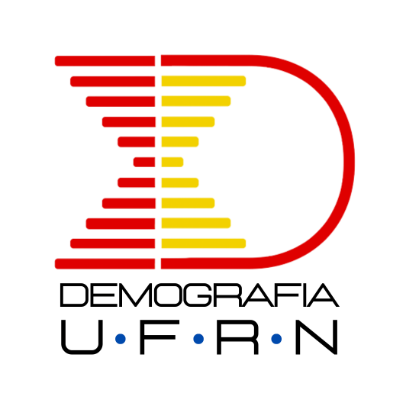
\includegraphics[width=0.9\linewidth]{figuras/logo_ppgdem.png}
        \end{minipage}
        
        \vspace{1.2cm}
        
        % Instituições
        {\large UNIVERSIDADE FEDERAL DE SERGIPE\par}
        {\large UNIVERSIDADE FEDERAL DO RIO GRANDE DO NORTE\par}
        
        \vspace{0.5cm}
        
        {\large PROGRAMA DE PÓS-GRADUAÇÃO EM DEMOGRAFIA\par}
        {\large DOUTORADO INTERINSTITUCIONAL EM POPULAÇÃO,\par}
        {\large ESTATÍSTICAS SOCIAIS E POLÍTICAS PÚBLICAS\par}
        
        \vspace{3cm}
        
        % Nome do aluno
        {\large \textbf{Andrés Ignácio Martínez Menéndez}\par}
        
        \vspace{3cm}
        
        % Título
        {\Large \textbf{Técnicas Demográficas I}\par}
        
        \vspace{0.6cm}
        
        {\large Trabalho 01\par}
  
        
        \vfill
        
        % Local e data
        {\small Aracaju (SE)\par}
        {\small Maio de 2026\par}
        
    \end{center}
\end{titlepage}
	
	\clearpage
	
	% -------------------------------------------------
	% Elementos pré-textuais (opcional)
	% -------------------------------------------------
	\tableofcontents
	\clearpage
	
	\listoffigures
	\clearpage
	
	\listoftables
	\clearpage
	
	
	
	\section*{Resumo}
	Este relatório apresenta os resultados

	\textbf{Palavras-chave:} demografia; .


	\section*{Abstract}
	This report presents the results 

	\textbf{Keywords:} demography; .
	\newpage

\section{INTRODUÇÃO}

A análise da distribuição da população por sexo e idade é um dos instrumentos
mais importantes da Demografia para compreender a estrutura e as transformações
de uma população ao longo do tempo. Por meio dela, é possível observar padrões
de fecundidade, mortalidade, envelhecimento e diferenças entre homens e
mulheres, elementos que ajudam a interpretar a dinâmica demográfica e a
subsidiar o planejamento de políticas públicas.

Neste trabalho, o foco é o Distrito Federal, utilizando dados oficiais do IBGE
extraídos do SIDRA e comparando os Censos Demográficos de 2010 e 2022. A partir
dessas bases, foi construída uma análise da população residente por sexo e
idade, com a padronização dos grupos etários em intervalos de 5 anos para permitir a
comparação entre os dois momentos censitários.

Além da organização e tratamento dos dados em Python, foram calculados
indicadores demográficos e produzidas visualizações gráficas para apoiar a
interpretação dos resultados. Entre os produtos elaborados estão as pirâmides
etárias, a distribuição percentual por grupos etários, a composição por grandes
grupos de idade e a razão de sexo por faixa etária. Com isso, busca-se
evidenciar as mudanças na estrutura etária do Distrito Federal entre 2010 e
2022, destacando tendências como o avanço do envelhecimento populacional e as
diferenças na composição por sexo ao longo das idades.

\section{METODOLOGIA}

Neste trabalho, a metodologia foi estruturada em quatro etapas: obtenção dos dados, tratamento e padronização da base,
cálculo de indicadores demográficos e geração de visualizações gráficas. Todo o processamento foi realizado em Python,
com uso das bibliotecas \texttt{pandas}, \texttt{requests}, \texttt{matplotlib} e \texttt{pathlib}, em uma estrutura de
projeto organizada para separar dados brutos, dados tratados e produtos gráficos.

\subsection{Obtenção dos dados}

Os dados utilizados são oficiais e foram extraídos do Sistema IBGE de Recuperação Automática (SIDRA), tomando como
recorte geográfico o Distrito Federal, identificado pelo código 53. Para o Censo Demográfico de 2022, foi utilizada a
tabela SIDRA 9514, que disponibiliza a população residente por sexo, idade e forma de declaração da idade. Para o Censo
Demográfico de 2010, foi utilizada a tabela SIDRA 3107, compatível com a análise por sexo e grupos de idade.
Conforme a documentação do próprio sistema, o SIDRA organiza e disponibiliza
tabelas estatísticas oficiais do IBGE em formato acessível para consulta e
download \cite{sidra_ibge_tabelas}.

A rotina de download foi implementada em Python no arquivo \texttt{baixar\_dados.py}. O programa consulta a API do SIDRA,
verifica o retorno da requisição e salva os arquivos brutos na pasta \texttt{dados/brutos}. Quando os arquivos já existem,
o script evita novo download, a menos que o usuário solicite atualização por meio da opção \texttt{--atualizar}. Essa
estratégia reduz retrabalho e facilita a reprodução da análise.

\subsection{Tratamento e padronização}

Após o download, os arquivos brutos foram tratados no arquivo \texttt{tratar\_dados.py}. Como as tabelas de 2010 e 2022
apresentam estruturas distintas, o tratamento foi feito por funções separadas. Em ambos os casos, a base foi padronizada
com as variáveis:

\begin{itemize}
    \item ano;
    \item uf;
    \item codigo\_uf;
    \item sexo;
    \item idade;
    \item grupo\_etario;
    \item populacao.
\end{itemize}

Para permitir a comparação entre os censos, as idades foram agrupadas em quinquênios:
0--4, 5--9, 10--14, 15--19, 20--24, 25--29, 30--34, 35--39, 40--44, 45--49,
50--54, 55--59, 60--64, 65--69, 70--74, 75--79 e 80 anos ou mais. Nos arquivos
tratados, os registros agregados foram organizados em formato longo, facilitando
os cálculos estatísticos e a geração dos gráficos.

Além da base tratada por ano, o processo também gera uma base consolidada com
os dois censos, salva em \texttt{dados/tratados/populacao\_df\_2010\_2022\_tratada.csv}.
Essa estrutura permite comparar os indicadores entre 2010 e 2022 de maneira
consistente.

\subsection{Indicadores demográficos}

Com a base tratada, foram calculados indicadores sintéticos para cada censo.
Entre eles estão a população total, a população masculina, a população feminina,
os percentuais por sexo, a razão de sexo, a população em três grandes grupos
etários (0 a 14 anos, 15 a 64 anos e 65 anos ou mais), os percentuais desses
grupos, o índice de envelhecimento e a razão de dependência.

Esses indicadores foram implementados no arquivo \texttt{indicadores.py} e
exportados para a pasta \texttt{dados/tratados} no arquivo
\texttt{indicadores\_df\_2010\_2022.csv}. A razão de sexo foi calculada como o
quociente entre homens e mulheres multiplicado por 100. O índice de
envelhecimento foi obtido pela razão entre a população de 65 anos ou mais e a
população de 0 a 14 anos, multiplicada por 100. Já a razão de dependência foi
calculada pela soma da população jovem e idosa dividida pela população em idade
potencialmente ativa, também multiplicada por 100.

As fórmulas utilizadas seguem a definição clássica apresentada por Grupo de
Foz~\cite{grupofoz2021metodos}. Em termos formais, a razão de sexo é dada por
\[
RS = \frac{H}{M} \times 100,
\]
em que \(H\) representa a população masculina e \(M\) a população feminina.

A distribuição percentual por sexo foi calculada por:
\[
\%H = \frac{H}{P} \times 100
\qquad \text{e} \qquad
\%M = \frac{M}{P} \times 100,
\]
em que \(P\) é a população total.

O índice de envelhecimento foi definido como:
\[
IE = \frac{P_{65+}}{P_{0-14}} \times 100,
\]
e a razão de dependência como:
\[
RD = \frac{P_{0-14} + P_{65+}}{P_{15-64}} \times 100.
\]
Nessas expressões, \(P_{0-14}\), \(P_{15-64}\) e \(P_{65+}\) correspondem,
respectivamente, às populações jovem, adulta e idosa.

\subsection{Visualizações gráficas}

As visualizações foram produzidas no arquivo \texttt{graficos.py} e salvas na
pasta \texttt{graficos}. Foram elaboradas pirâmides etárias para 2010 e 2022,
com homens à esquerda e mulheres à direita, além de gráficos comparativos da
distribuição percentual por grupos etários, da composição por grandes grupos de
idade e da razão de sexo por grupo etário.

A construção dos gráficos seguiu a lógica demográfica usual, com os grupos
etários organizados em ordem crescente no eixo vertical e as barras de homens
representadas com valores negativos para permitir a simetria visual da
pirâmide. Também foram incluídos título, legenda e fonte dos dados em cada
figura, de modo a facilitar a leitura e a interpretação dos resultados.

\subsection{Fluxo de execução}

O arquivo \texttt{main.py} centraliza o fluxo do programa. A execução segue a
ordem: baixar os dados, tratar as bases, calcular os indicadores, gerar as
tabelas comparativas e produzir os gráficos. Essa organização torna o processo
reprodutível e facilita a atualização futura caso novas versões dos dados do
IBGE sejam disponibilizadas.

Por fim, os produtos finais foram encaminhados para o relatório em LaTeX por
meio dos arquivos gerados automaticamente pelo script em Python, permitindo
manter os dados, as tabelas e as figuras sincronizados com a análise apresentada
neste documento. Todo o código-fonte, os arquivos de dados tratados e os
gráficos produzidos estão disponíveis no repositório
\href{https://github.com/ammenendez/TD-01.git}{ammenendez/TD-01.git}.

\section{RESULTADOS}



\subsection{Evolução da população total e da composição por sexo}

Os indicadores resumidos na Tabela~\ref{tab:indicadores_df} mostram que a
população do Distrito Federal aumentou de 2.570.160 habitantes em 2010 para
2.817.381 em 2022, o que representa um crescimento absoluto de 247.221 pessoas
no período. Embora a população total tenha aumentado, a participação relativa
de homens e mulheres permaneceu bastante estável, com leve predomínio feminino
nos dois censos.

\begin{table}[H]
\small
\centering
\caption{Indicadores demográficos do Distrito Federal, 2010 e 2022.}
\label{tab:indicadores_df}
\begin{tabular}{lrr}
\toprule
Indicador & 2010 & 2022 \\
\midrule
\multicolumn{3}{l}{\textbf{População observada}} \\
População total & 2.570.160 & 2.817.381 \\
População masculina & 1.228.880 & 1.342.786 \\
População feminina & 1.341.280 & 1.474.595 \\
População de 0 a 14 anos & 796.943 & 789.312 \\
População de 15 a 64 anos & 1.646.261 & 1.781.213 \\
População de 65 anos ou mais & 126.956 & 246.856 \\
\midrule
\multicolumn{3}{l}{\textbf{Indicadores calculados}} \\
Percentual masculino (\%) & 47,81 & 47,66 \\
Percentual feminino (\%) & 52,19 & 52,34 \\
Razão de sexo & 91,62 & 91,06 \\
Percentual de jovens (\%) & 31,01 & 28,02 \\
Percentual de adultos (\%) & 64,05 & 63,22 \\
Percentual de idosos (\%) & 4,94 & 8,76 \\
Índice de envelhecimento & 15,93 & 31,27 \\
Razão de dependência & 56,12 & 58,17 \\
\bottomrule
\end{tabular}
\end{table}

Em 2010, os homens representavam 47,81\% da população e as mulheres 52,19\%.
Em 2022, esses percentuais passaram para 47,66\% e 52,34\%, respectivamente.
A razão de sexo caiu de 91,62 homens para cada 100 mulheres, em 2010, para
91,06 em 2022, indicando manutenção de um padrão de maior presença feminina no
conjunto da população.

\subsection{Estrutura etária e envelhecimento}

A comparação entre os dois censos, sintetizada na Tabela~\ref{tab:indicadores_df},
evidencia uma mudança importante na estrutura etária do Distrito Federal. A
população de 0 a 14 anos passou de 796.943 pessoas em 2010 para 789.312 em
2022, o que reduziu sua participação relativa de 31,01\% para 28,02\%. Em
contrapartida, a população de 65 anos ou mais saltou de 126.956 para 246.856
pessoas, passando de 4,94\% para 8,76\% do total da população.

Esse movimento é sintetizado pelo índice de envelhecimento, que subiu de 15,93
em 2010 para 31,27 em 2022. A razão de dependência também aumentou, passando de
56,12 para 58,17. Esses resultados indicam que o Distrito Federal vem passando
por um processo de envelhecimento populacional, ainda que a proporção de
população em idade potencialmente ativa continue majoritária.

\subsection{Pirâmides etárias}

As pirâmides etárias confirmam visualmente as mudanças observadas nos
indicadores. Em 2010, a estrutura etária ainda apresentava uma base mais larga,
indicando maior presença de crianças e adolescentes. Já em 2022, a base se
apresenta mais estreita, enquanto as faixas adultas e idosas ganham maior
expressão relativa. Esse formato é compatível com a transição demográfica em
curso e com a redução da participação dos grupos mais jovens.

Além disso, a distribuição por sexo mostra maior equilíbrio nas idades adultas,
mas com aumento da predominância feminina nas idades mais avançadas, o que é
compatível com a maior sobrevivência feminina observada em diferentes contextos
demográficos.



\subsection{Distribuição percentual por grupos etários}

A comparação dos grupos quinquenais entre 2010 e 2022, apresentada nas Figuras
\ref{fig:piramide_2010}, \ref{fig:piramide_2022} e
\ref{fig:distribuicao_percentual}, reforça o deslocamento da estrutura etária
para faixas mais envelhecidas. Os grupos mais jovens perderam participação
relativa, enquanto grupos intermediários e idosos passaram a ocupar parcelas
maiores da população.

\begin{figure}[H]
    \centering
    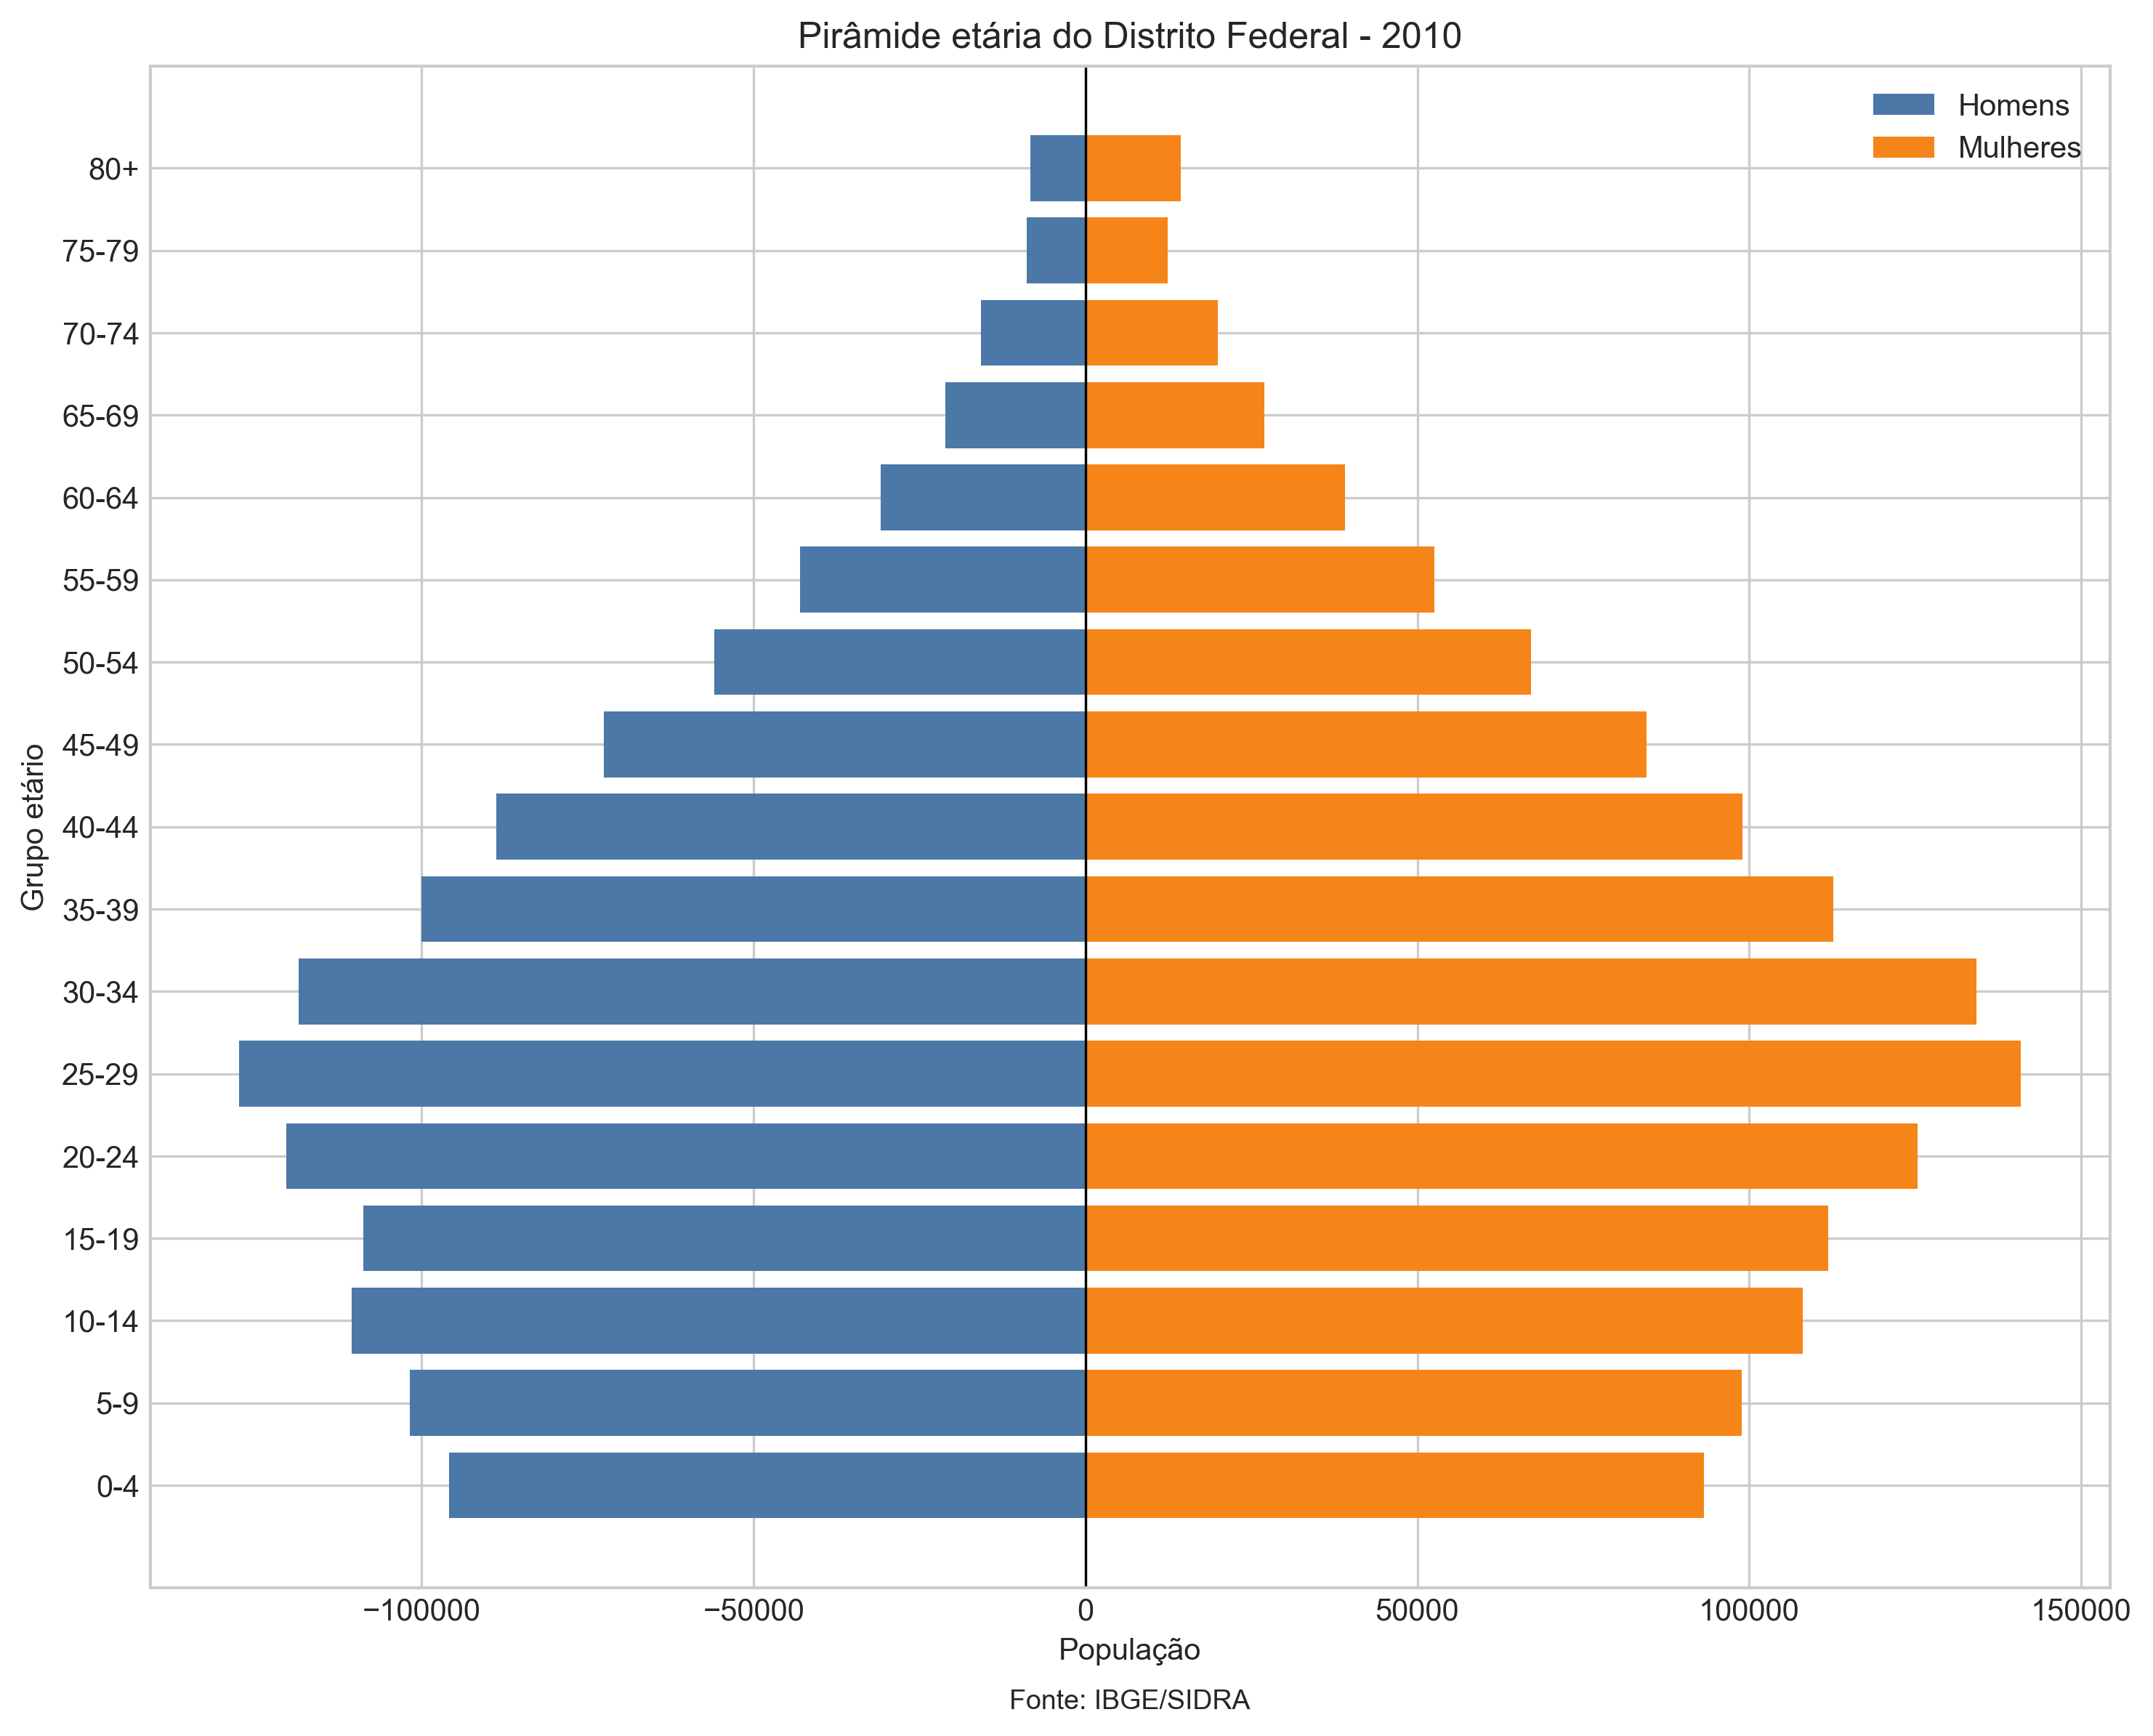
\includegraphics[width=0.88\textwidth]{../graficos/piramide_etaria_df_2010.png}
    \caption{Pirâmide etária do Distrito Federal em 2010.}
    \label{fig:piramide_2010}
\end{figure}

\begin{figure}[H]
    \centering
    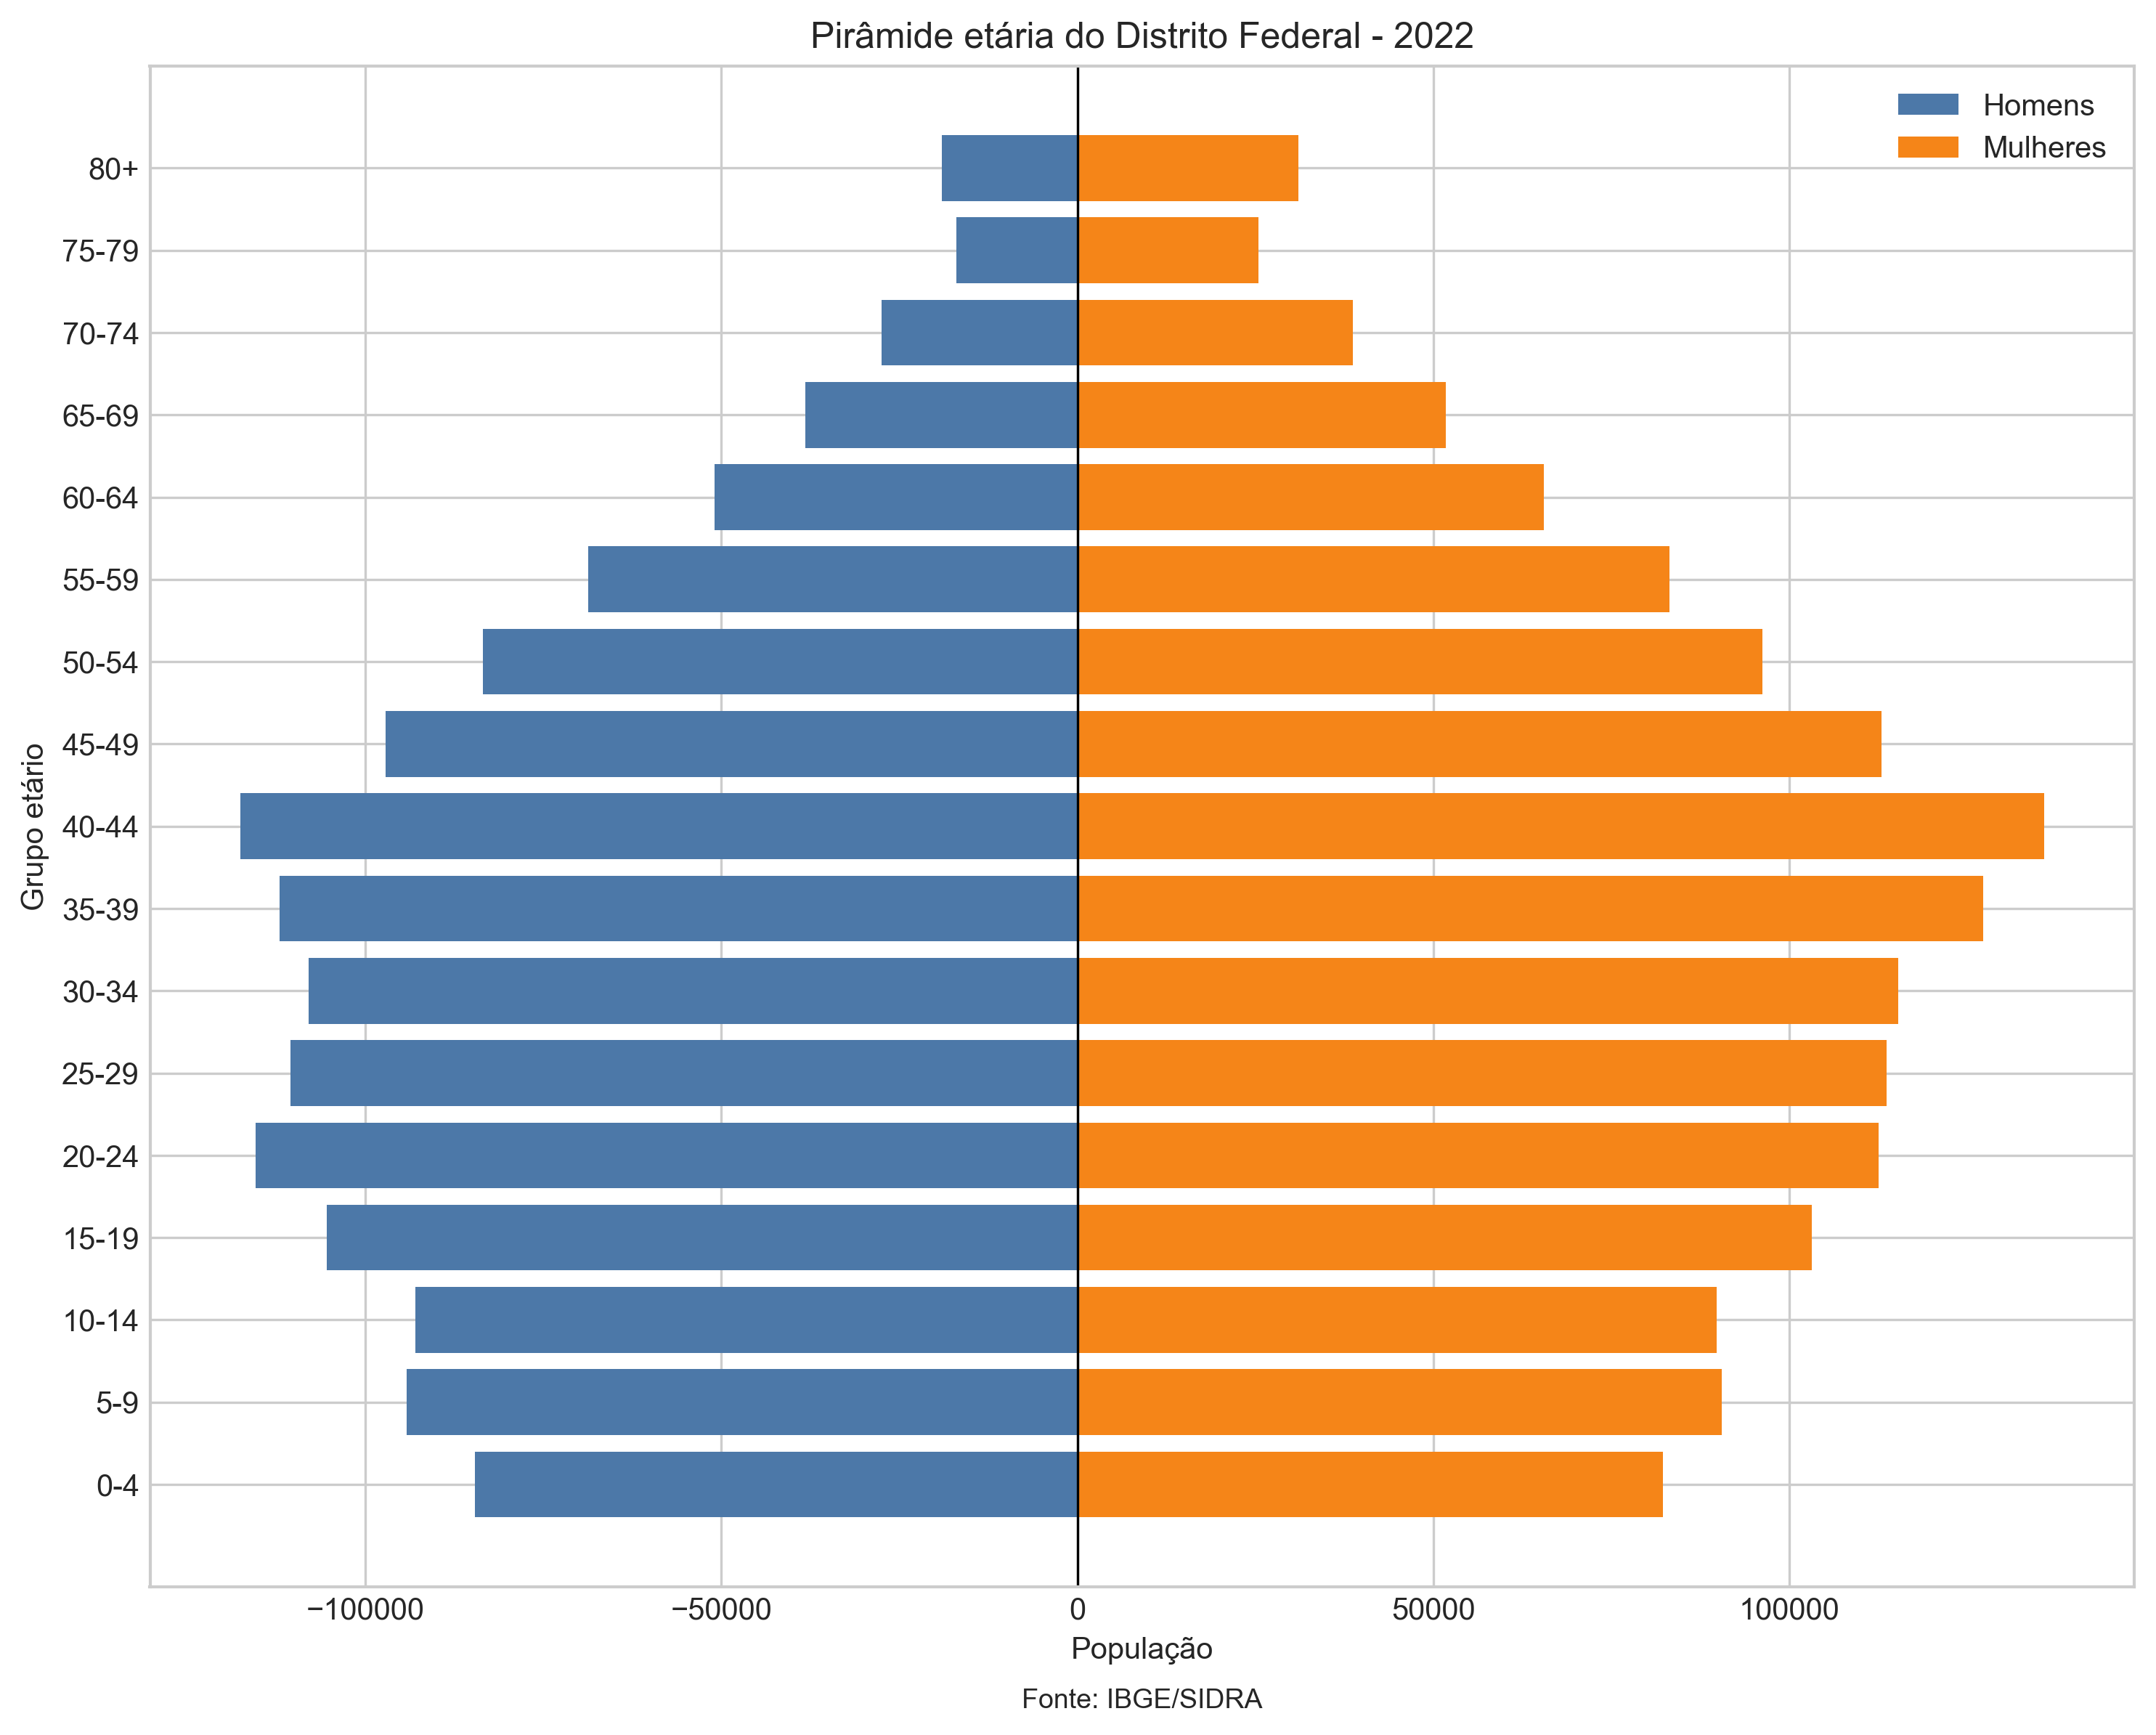
\includegraphics[width=0.88\textwidth]{../graficos/piramide_etaria_df_2022.png}
    \caption{Pirâmide etária do Distrito Federal em 2022.}
    \label{fig:piramide_2022}
\end{figure}

Esse padrão pode ser observado tanto na distribuição percentual por grupos
etários, na Figura~\ref{fig:distribuicao_percentual}, quanto no gráfico de
barras com os grandes grupos de idade, na Figura~\ref{fig:jovens_adultos_idosos}.
Em 2010, a população jovem ainda tinha peso considerável, mas em 2022 a
presença relativa dos idosos se ampliou, confirmando a tendência de
envelhecimento da população do Distrito Federal.

\begin{figure}[H]
    \centering
    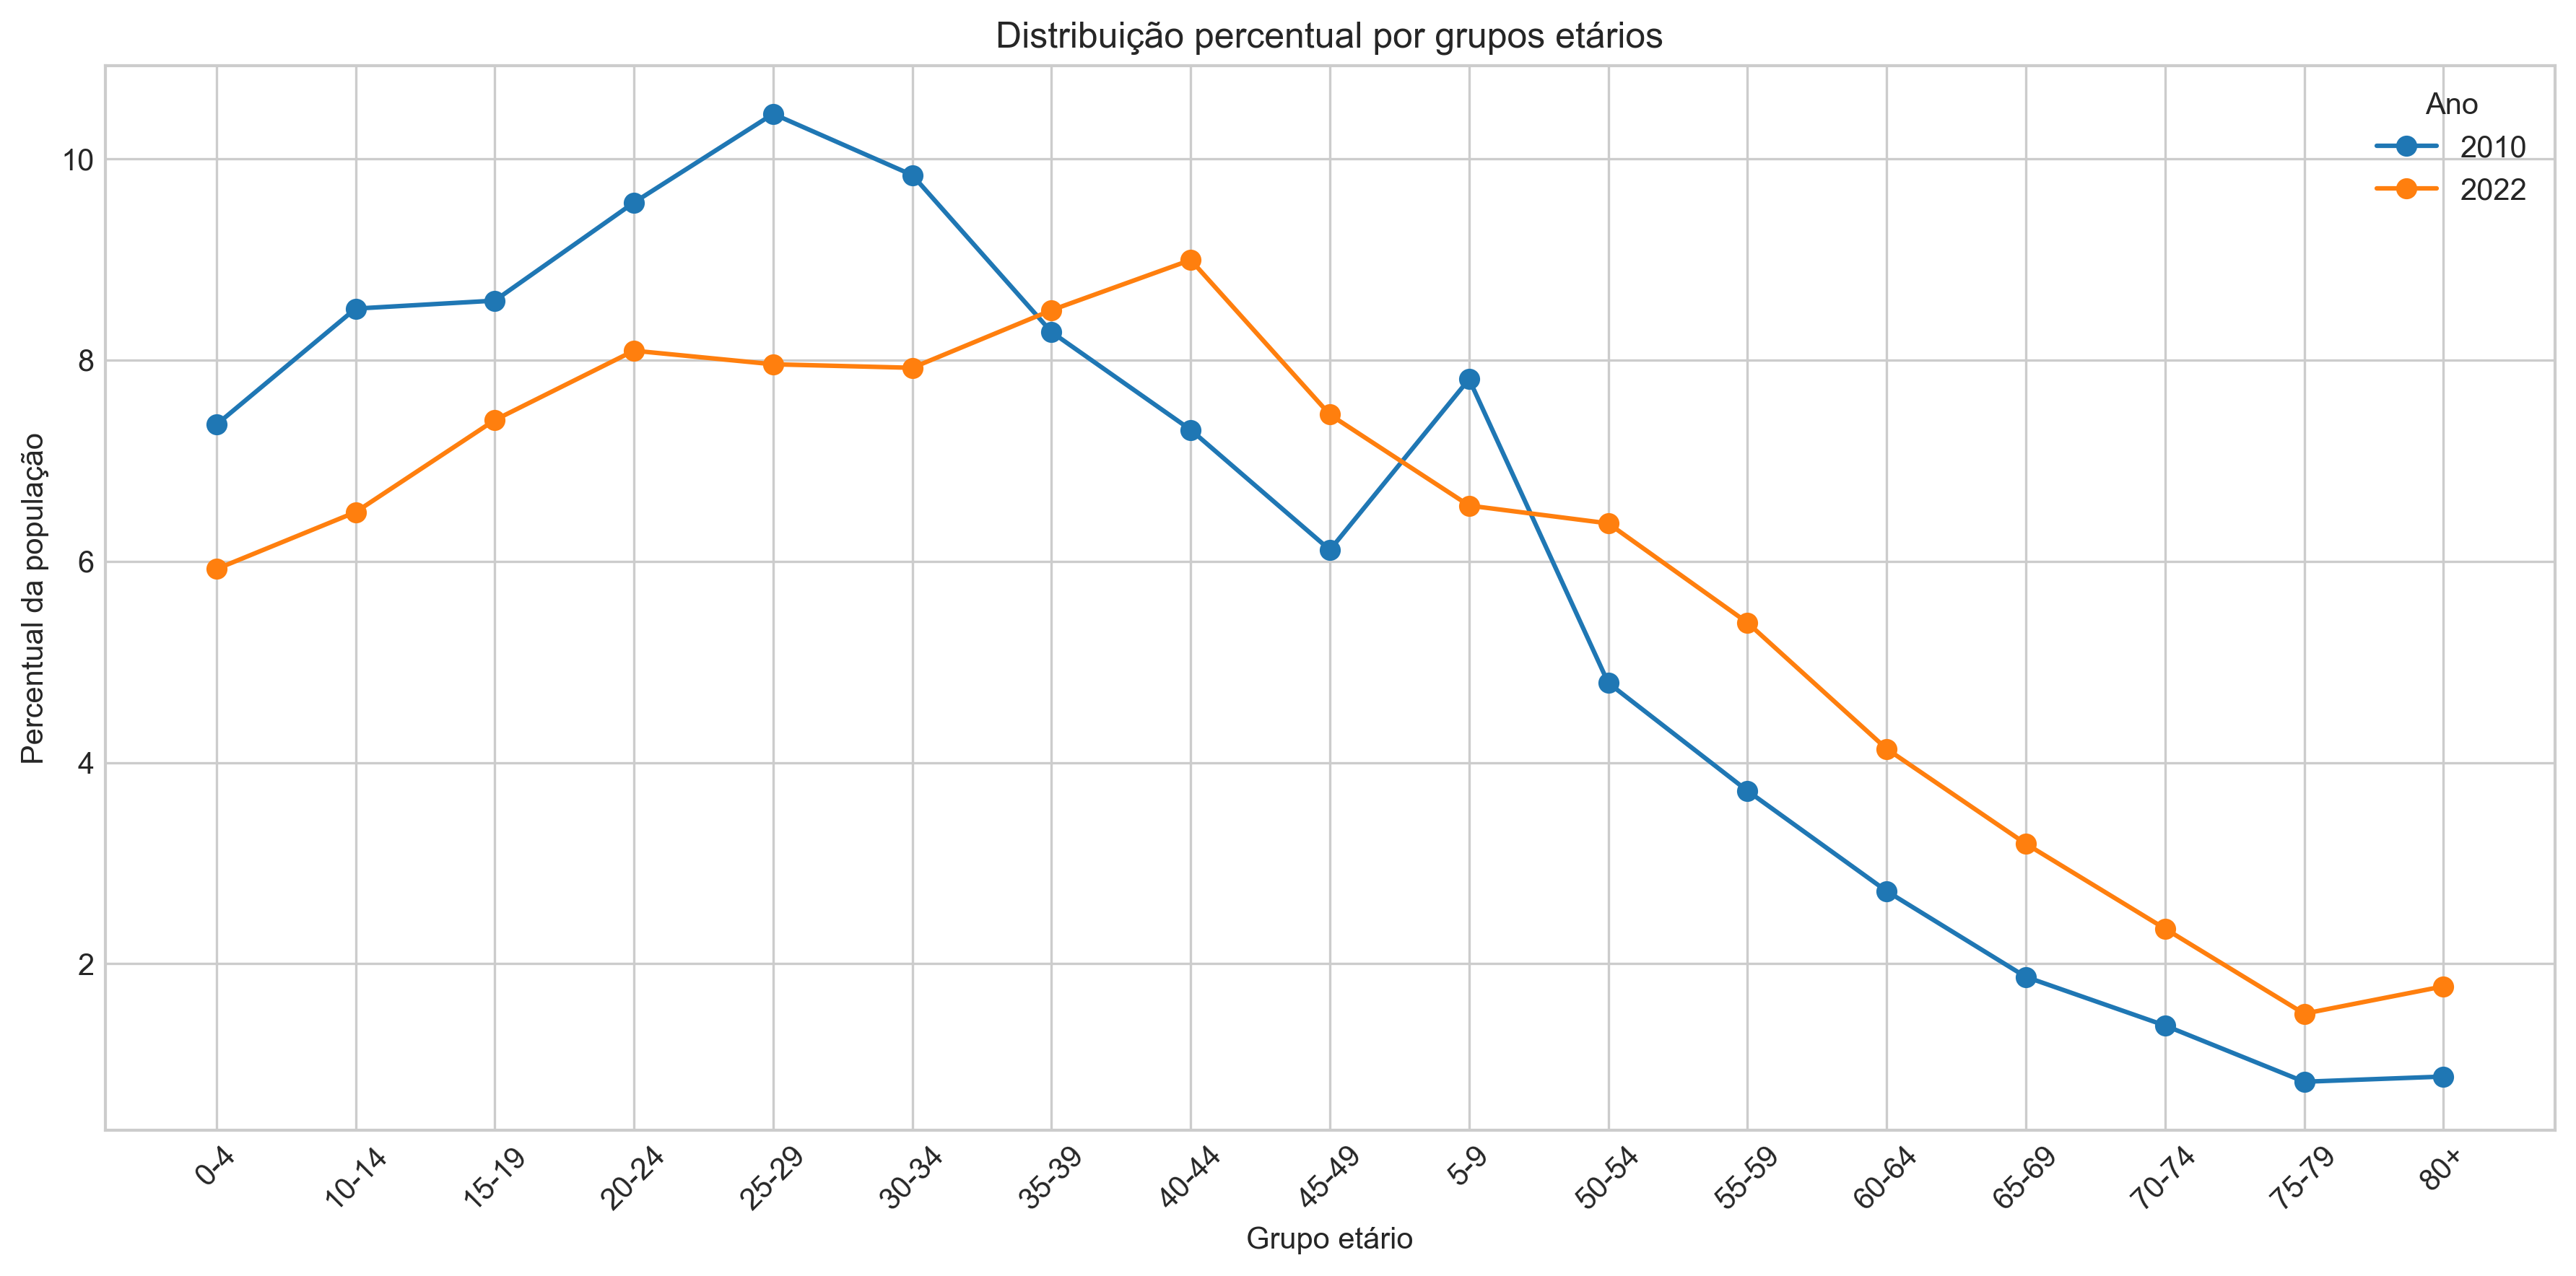
\includegraphics[width=0.88\textwidth]{../graficos/distribuicao_percentual_grupos_etarios_2010_2022.png}
    \caption{Distribuição percentual da população do Distrito Federal por grupos etários, 2010 e 2022.}
    \label{fig:distribuicao_percentual}
\end{figure}

\begin{figure}[H]
    \centering
    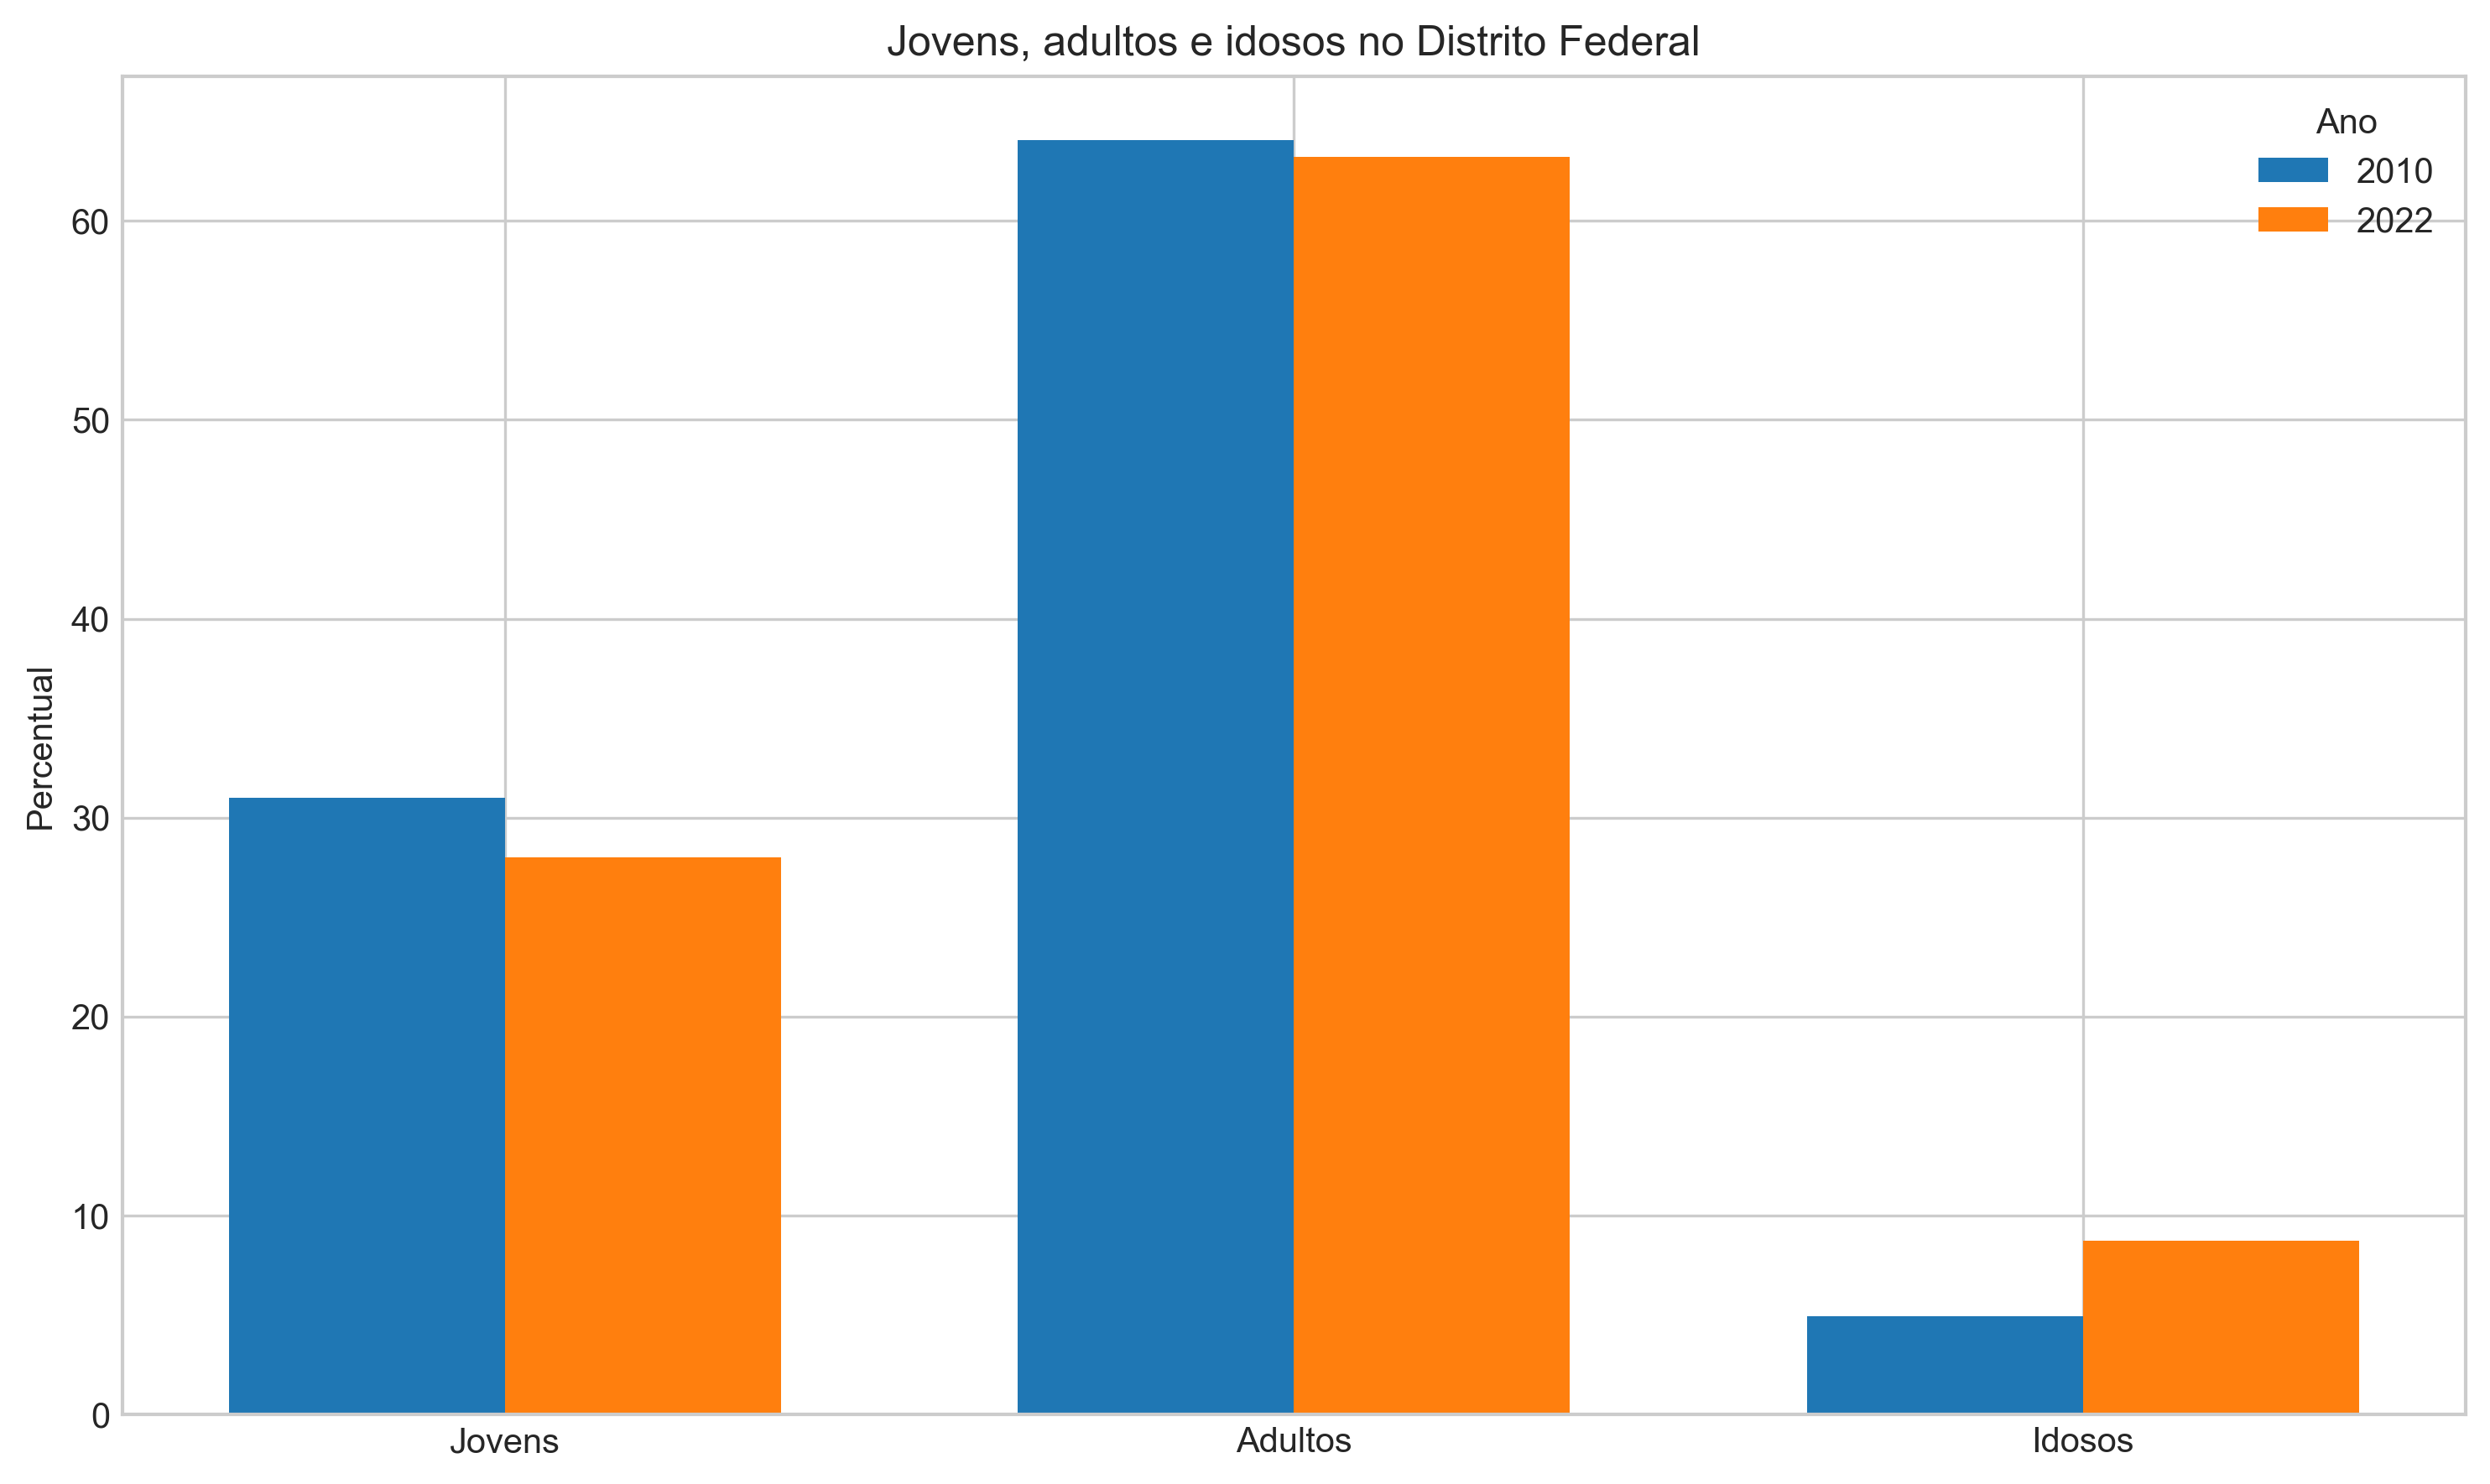
\includegraphics[width=0.88\textwidth]{../graficos/jovens_adultos_idosos_2010_2022.png}
    \caption{Comparação entre jovens, adultos e idosos no Distrito Federal, 2010 e 2022.}
    \label{fig:jovens_adultos_idosos}
\end{figure}

\subsection{Razão de sexo por grupo etário}

A razão de sexo por grupo etário, mostrada na Figura~\ref{fig:razao_sexo_grupo_etario},
mostra diferenças importantes ao longo do ciclo de vida. Nos grupos mais
jovens, a relação entre homens e mulheres tende a ser mais equilibrada, com
pequenas oscilações entre os censos. A partir das idades mais elevadas, a razão
de sexo diminui, evidenciando maior presença feminina nas faixas etárias
avançadas.

Esse comportamento é esperado em uma população em processo de envelhecimento,
uma vez que a mortalidade masculina costuma ser mais elevada ao longo da vida,
produzindo um desequilíbrio progressivo entre os sexos nas idades adultas e
idosas. No Distrito Federal, esse padrão aparece com clareza ao comparar 2010 e
2022.

\begin{figure}[H]
    \centering
    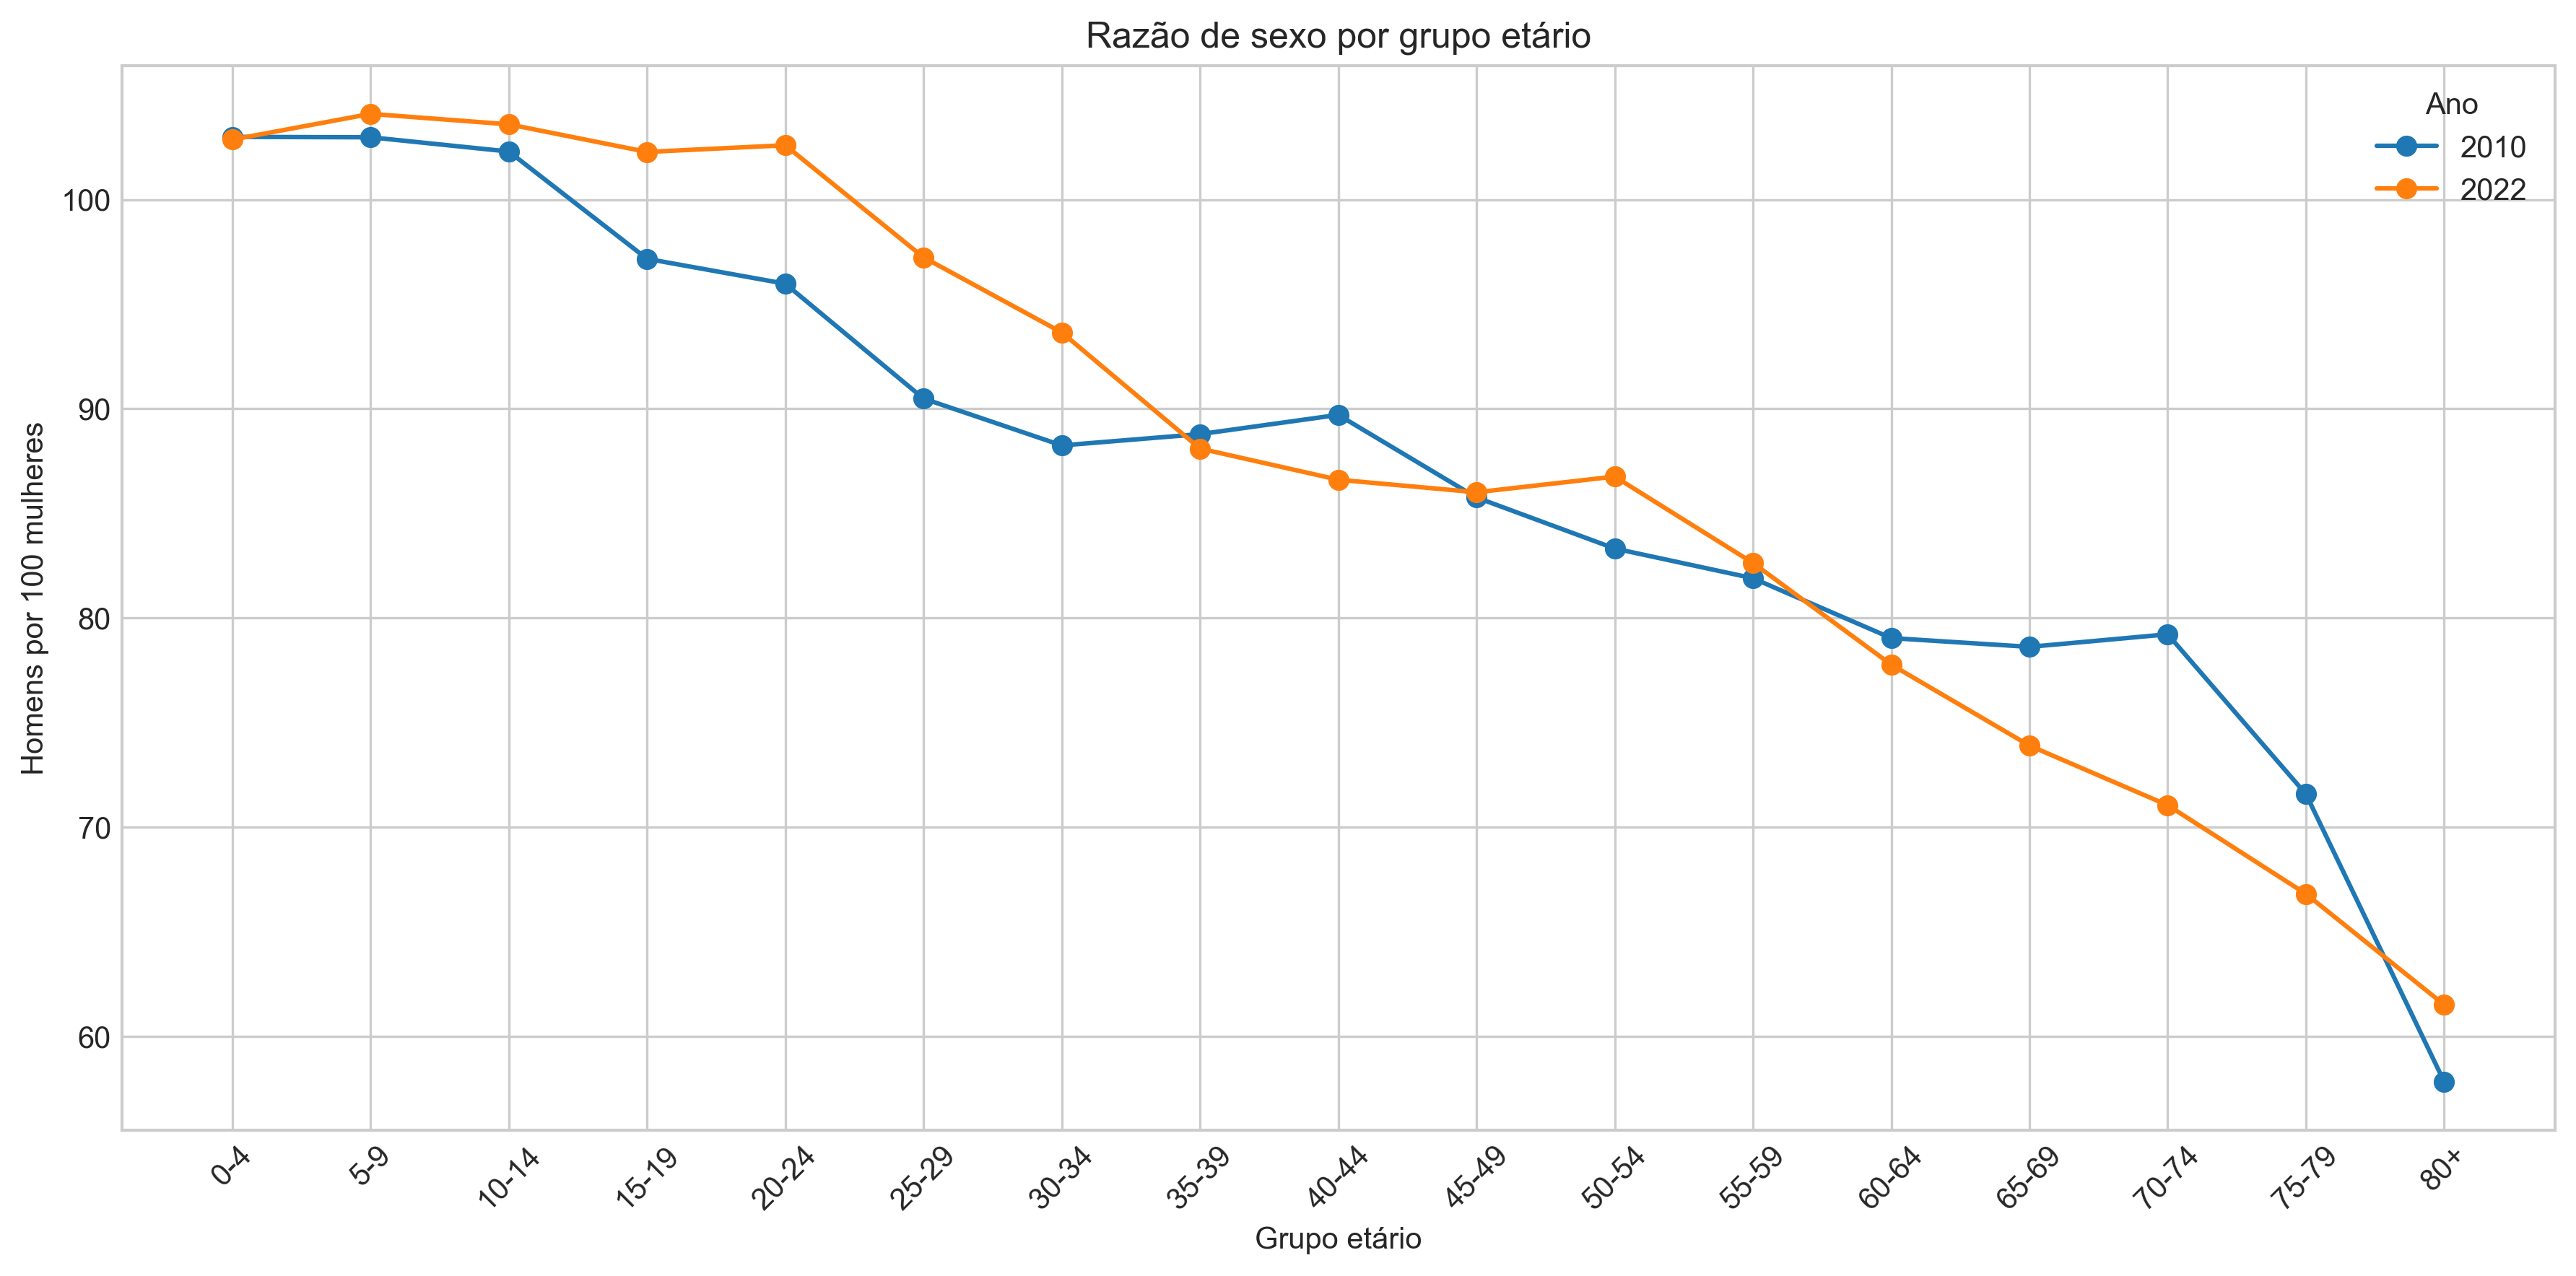
\includegraphics[width=0.92\textwidth]{../graficos/razao_sexo_por_grupo_etario.png}
    \caption{Razão de sexo por grupo etário no Distrito Federal, 2010 e 2022.}
    \label{fig:razao_sexo_grupo_etario}
\end{figure}






\section{CONSIDERAÇÕES FINAIS}

Este trabalho teve como objetivo analisar a população do Distrito Federal por
sexo e idade, comparando os Censos Demográficos de 2010 e 2022 com base em
dados oficiais do IBGE/SIDRA. A partir do tratamento dos arquivos brutos em
Python, foi possível organizar a base de forma padronizada, calcular
indicadores demográficos e produzir visualizações que facilitam a leitura da
estrutura populacional.

Os resultados mostraram crescimento da população total no período, acompanhando
alterações importantes na composição etária. A redução da participação relativa
de crianças e adolescentes, associada ao aumento da população idosa e do índice
de envelhecimento, evidencia o avanço da transição demográfica no Distrito
Federal. Embora a população em idade potencialmente ativa continue majoritária,
o aumento da razão de dependência sinaliza maior pressão futura sobre as faixas
etárias economicamente ativas.

As pirâmides etárias, a distribuição percentual por grupos etários e a razão de
sexo por faixa etária reforçaram visualmente esses achados, permitindo observar
que o Distrito Federal apresenta uma estrutura etária em processo de
amadurecimento, com maior participação feminina nas idades avançadas. Assim, os
indicadores e gráficos elaborados não apenas descrevem a situação demográfica,
mas também ajudam a interpretar as mudanças estruturais ocorridas entre 2010 e
2022.

Do ponto de vista metodológico, o trabalho também contribuiu para consolidar a
utilização de Python como ferramenta de coleta, tratamento, análise e
visualização de dados demográficos, organizando um fluxo reprodutível que pode
ser atualizado em novas versões da base do IBGE.
\newpage
\bibliography{references}

\end{document}
